\section{Peripherals}
\label{sec:periphs}

In order to controll the Basys 2 board peripherals with the picoversat controller, peripheral drivers are used. The pheripherals are mapped in memmory, refer to the memory map in section~\ref{sec:mem_map} to check the peripheral's addresses.

\subsection{General Purpose Register File}

This peripheral contains a 16x32bit register file that can be used by user
programs. Refer to the picoversat manual for more information about this peripheral. 

\subsection{Debug Printer}

This peripheral can be used by user programs to print characters, mainly for
debug purposes. Refer to the picoversat manual for more information about this peripheral.

\subsection{Sequencer Loop Controller}

This peripheral is used to generate the sequencer loop. The loop and note frequency can be set by using the \textit{freq} input and by selecting the according selector signal.
The Sequencer loop controller will output a square wave corresponding to the loop ouput. The led outputs are directly connected to the LED driver peripheral and send information about the current note. 

\begin{figure}[!htbp]
    \centerline{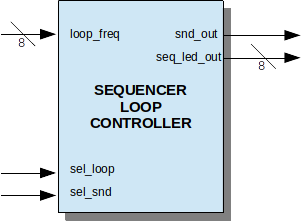
\includegraphics[scale=0.5]{SequencerLoopcontroler.png}}
    \vspace{0cm}\caption{PicoVersat SoC with two peripherals}
    \label{fig:periphs}
\end{figure}

% Please add the following required packages to your document preamble:
% \usepackage{booktabs}
\begin{table}[!htbp]
    \centering
    \caption{Sequencer Loop Controller Inputs}
    \label{tab:slcIn}
    \begin{tabular}{@{}lcl@{}}
    \toprule
    Name      & \multicolumn{1}{l}{\#bits} & Description                                    \\ \midrule
    freq & 8                          & Loop Period / Note Frequency                                    \\
    sel\_loop & 1                          & Loop period select signal (address decoder)    \\
    sel\_snd  & 1                          & Note frequency select signal (address decoder) \\ \bottomrule
    \end{tabular}
    \end{table}

    % Please add the following required packages to your document preamble:
% \usepackage{booktabs}
\begin{table}[!htbp]
    \centering
    \caption{Sequencer Loop Controller Outputs}
    \label{tab:slcOut}
    \begin{tabular}{@{}lcl@{}}
    \toprule
    Name          & \multicolumn{1}{l}{\#bits} & Description             \\ \midrule
    snd\_out      & 1                          & Audio Output            \\
    seq\_led\_out & 8                          & Current note led output \\ \bottomrule
    \end{tabular}
    \end{table}

\subsection{LED Driver}

The LED driver will display the current note. The input of the driver is directly controlled by the sequencer loop controller.

\begin{figure}[!htbp]
    \centerline{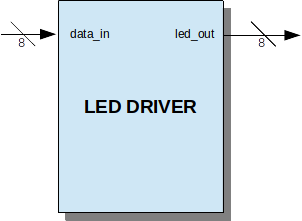
\includegraphics[scale=0.5]{led_drive_blk.png}}
    \vspace{0cm}\caption{PicoVersat SoC with two peripherals}
    \label{fig:periphs}
\end{figure}

% Please add the following required packages to your document preamble:
% \usepackage{booktabs}
\begin{table}[!htbp]
    \centering
    \caption{Led driver inputs}
    \label{tab:ledIn}
    \begin{tabular}{@{}lll@{}}
    \toprule
    Name     & \#bits                & Description             \\ \midrule
    data\_in & \multicolumn{1}{c}{8} & Led display information \\ \bottomrule
    \end{tabular}
    \end{table}

% Please add the following required packages to your document preamble:
% \usepackage{booktabs}
\begin{table}[!htbp]
    \centering
    \caption{Led driver outputs}
    \label{tab:ledOut}
    \begin{tabular}{@{}lll@{}}
    \toprule
    Name     & \#bits                & Description        \\ \midrule
    led\_out & \multicolumn{1}{c}{8} & Led display output \\ \bottomrule
    \end{tabular}
    \end{table}



\subsection{Switch Driver}

This driver reads the state of the slide-switches of the Basys 2 board.

\begin{figure}[!ht]
    \centerline{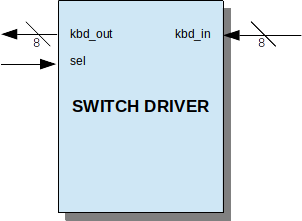
\includegraphics[scale=0.5]{sw_drive_blk.png}}
    \vspace{0cm}\caption{PicoVersat SoC with two peripherals}
    \label{fig:periphs}
\end{figure}

% Please add the following required packages to your document preamble:
% \usepackage{booktabs}
\begin{table}[ht]
    \centering
    \caption{Switch driver inputs}
    \label{tab:swIn}
    \begin{tabular}{@{}lcl@{}}
    \toprule
    Name   & \multicolumn{1}{l}{\#bits} & Description                       \\ \midrule
    sw\_in & 8                          & Switch state inputs               \\
    sel    & 1                          & driver selector (address decoder) \\ \bottomrule
    \end{tabular}
    \end{table}

    % Please add the following required packages to your document preamble:
% \usepackage{booktabs}
\begin{table}[ht]
    \centering
    \caption{Switch driver outputs}
    \label{tab:swOut}
    \begin{tabular}{@{}lll@{}}
    \toprule
    Name     & \#bits                & Description          \\ \midrule
    kbd\_out & \multicolumn{1}{c}{8} & Switch state outputs \\ \bottomrule
    \end{tabular}
    \end{table}



\subsection{Push-Button Driver}

This driver reads the state of the push-buttons of the Basys 2 board.



\begin{figure}[!htbp]
    \centerline{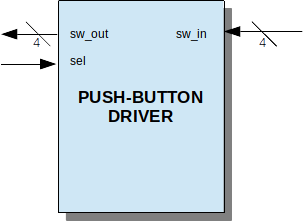
\includegraphics[scale=0.5]{push_drive_blk.png}}
    \vspace{0cm}\caption{PicoVersat SoC with two peripherals.}
    \label{fig:periphs}
\end{figure}

% Please add the following required packages to your document preamble:
% \usepackage{booktabs}
\begin{table}[!htbp]
    \centering
    \caption{Push-button driver inputs}
    \label{tab:pshIn}
    \begin{tabular}{@{}lcl@{}}
    \toprule
    Name   & \multicolumn{1}{l}{\#bits} & Description                       \\ \midrule
    sw\_in & 4                          & Push-button state inputs              \\
    sel    & 1                          & Driver selector (address decoder) \\ \bottomrule
    \end{tabular}
    \end{table}

% Please add the following required packages to your document preamble:
% \usepackage{booktabs}
\begin{table}[!htbp]
    \centering
    \caption{Push-button driver outputs}
    \label{tab:pshOut}
    \begin{tabular}{@{}lll@{}}
    \toprule
    Name    & \#bits                & Description               \\ \midrule
    sw\_out & \multicolumn{1}{c}{4} & Push-button state outputs \\ \bottomrule
    \end{tabular}
    \end{table}

The peripheral are interconnected according to the following picture:

\begin{figure}[!htbp]
    \centerline{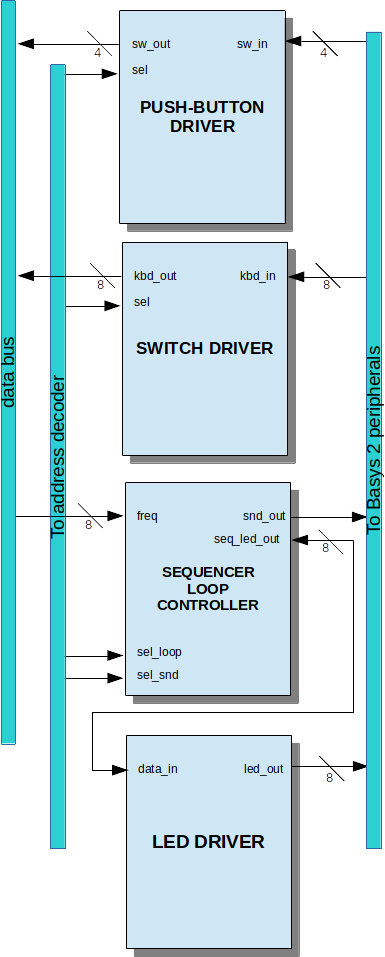
\includegraphics[scale=0.5]{periphs_interconn.png}}
    \vspace{0cm}\caption{Peripherals interconnections.}
    \label{fig:periphs}
\end{figure}
